\chapter{Leveraging structured forest for segmentation}
\label{Chapter4}
Given an edge detection result, various methods could be employed to obtain image segmentation.  One approach is to try and identify all possible boundaries of segmentation regions, based on the probability of boundary score produced by the edge detector. Those boundaries finely partition the image pixel graph. The regions closed by them constitute an oversegmentation of the image. Different tasks require segmentation at different level of detail. It is useful, therefore, to be able to obtain coarser segmentations as well. By reasoning about the salience of region boundaries, one could construct a hierarchy of segmentations. Going up the hierarchy corresponds to coarsening the segmentation by merging neighbouring regions which are separated by a weak boundary. To establish the order in which to merge the regions, we must be able to tell weak from strong boundaries. We want to associate a score with every possible region boundary, which score should reflect the strength of that intervening boundary.

\textbf{Structured voting:} To score the region boundaries we take a patch comparison approach. The edge detector which we employ, Structured edge (SE) by Dollar et al.~\cite{DollarICCV13edges}, associates a segmentation patch centred around every pixel location in the image - its most likely segmentation. The possible region boundaries locations are obtained by a watershed transformation on the output of this detector. For the same location we attain a patch from the watershed locations image. We then explore strategies to compare those two patches and score the similarity between them, a higher score meaning higher local evidence for boundary. We call those \textbf{watershed weighting strategies}. The choice of such an approach defines how we conduct our \textbf{Structured voting (SV)}.

\textbf{How to vote? Two essentials:} We identify two important points in order to be able to score the two patches just described. Firstly, one being a local segmentation, and the other - a local oversegmentation, they are quite dissimilar. Therefore, one patch needs to be sensibly transformed, so that the two patches are comparable. Secondly, given that the two patches are comparable, what scoring function should be employed? We cast the problem of comparing two segmentation patches as a segmentation benchmark problem. Various boundary- and region-based metrics have been proposed for the task of evaluating image segmentation. We analyse the theoretical properties of some, and use a reasonable subset of them in our practical experiments. So a watershed weighting strategy has two aspects - making the patches sufficiently similar to compare, and choosing a scoring function to compare them.

In the terms of the framework of Arbelaez et al.\cite{Arbelaez11} - gPb-OWT-UCM, we propose to use SE instead of gPb as an edge detector. Further, we replace the Oriented watershed transform (OWT) by SV to obtain scored region boundary locations. Our image segmentation pipeline could then be titled SE-SV-UCM.

\begin{figure}[ht!]
\centering
 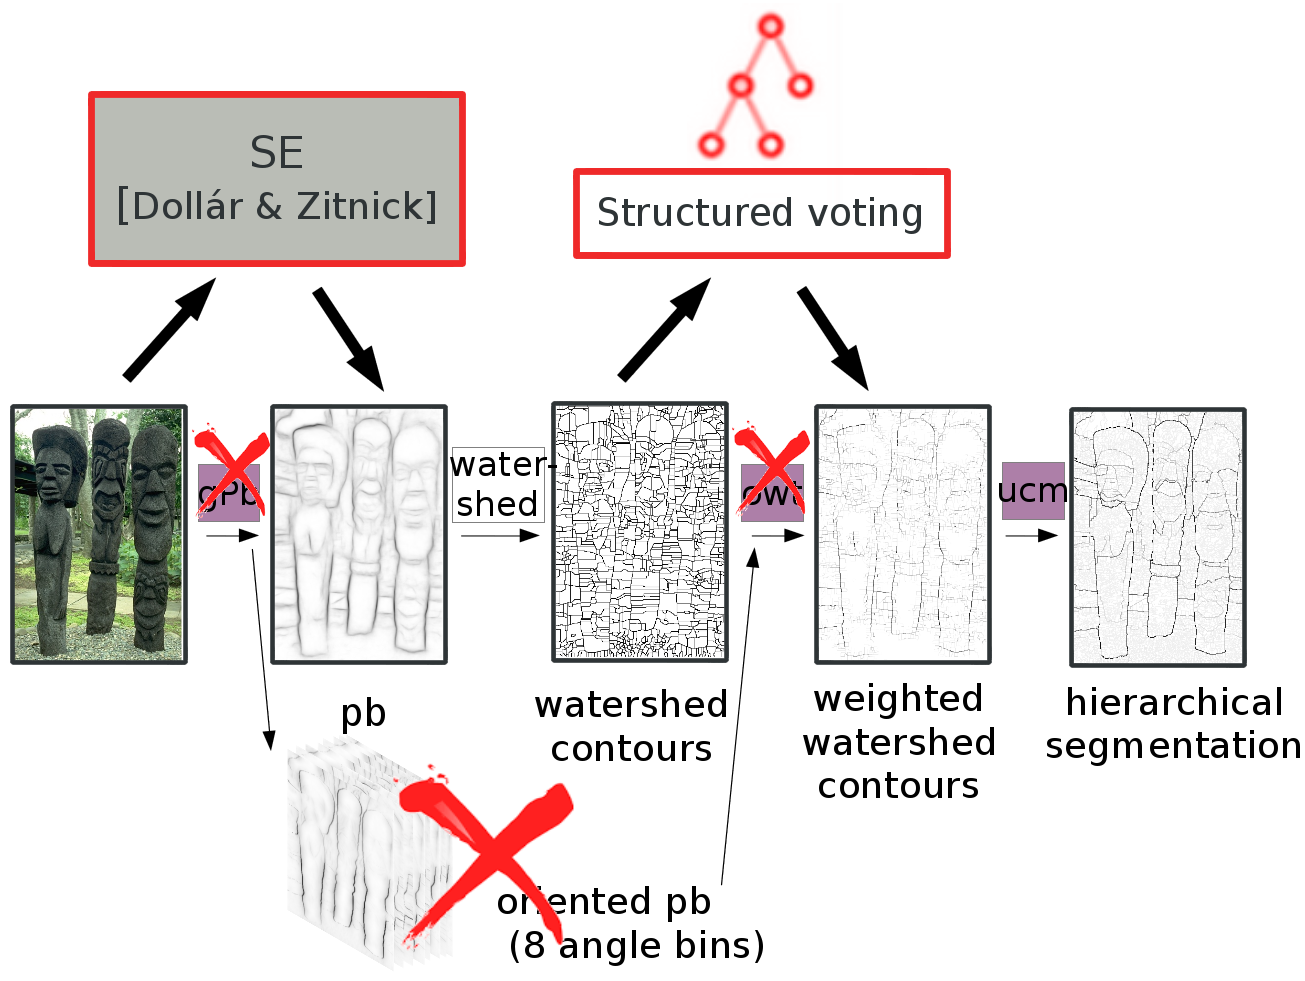
\includegraphics[width=1\textwidth]{images/SE-SV-UCM/SE-SV-UCM_pipeline.png}
\caption{Our SE-SV-UCM algorithm in the context of gPb-OWT-UCM pipeline.}
\label{fig:SE-SV-UCM-pipeline}
\end{figure}

\section{First stage of the pipeline - Edge detection - SE}
\textbf{gPb vs. structured edge}

\section{Second stage of the pipeline - Structured voting}

\textbf{Weighting the watershed locations}
\subsection{Comparing a structured forest patch to a watershed patch}
\subsubsection{Patch transformations}
\subsection{Scoring functions for patch similarity}
\subsubsection{Cast as a segmentation benchmark problem}
\subsubsection{Boundary and region metrics}
\label{boundary-and-region-metrics-maths}
\paragraph{BPR}
\label{BPR-maths}
\[
P=\frac{\left|S\cap\left(\bigcup\limits _{i=1}^{M}G_{i}\right)\right|}{|S|}
\]
\[
R=\frac{{\sum\limits _{i=1}^{M}\left|S\cap G_{i}\right|}}{\sum\limits _{i=1}^{M}\left|G_{i}\right|}
\]
\[
F=\frac{2PR}{P+R}
\]


where $S$ and $\{G_{i}\}_{i=1}^{M}$ are boundary maps and $\cap$
does a bipartite graph assignment between them.


\paragraph{RI (Rand Index)}


\subparagraph*{RI}

between two segmentations

\begin{align*}
RI(S,G) & =\frac{1}{T}\sum\limits _{j<k}\left[\mathbb{I}\left(S(j)=S(k)\wedge G(j)=G(k)\right)+\mathbb{I}\left(S(j)\neq S(k)\wedge G(j)\neq G(k)\right)\right]\\
 & =\frac{1}{T}\sum\limits _{(j,k)\in A}\left[c_{jk}\mathbb{I}\left(G(j)=G(k)\right)+(1-c_{jk})\mathbb{I}\left(G(j)\neq G(k)\right)\right]
\end{align*}


where $\mathbb{I}$ - the identity function,

$S(j)$ - the label of pixel $j$ in the segmentation $S$,

$c_{jk}=\mathbb{I}\left(S(j)=S(k)\right)$ - the event of the pair
of pixels $j$ and $k$ having the same label in segmentation $S$,

$A=\{(j,k)|j<k\}$ - the set of unique pairs of pixels,

$N=\left|S\right|=\left|G\right|$ - the number of pixels in the image
(and each segmentation), and 

$T=|A|=\binom{N}{2}$ - the number of possible unique pairs among
$N$ pixels.


\subparagraph*{RIMC (Random Index Monte Carlo)} %RSRI (Random Subsample RI)} previously CPD (Crude Patch Distance), which was a misnomer
\label{RIMC-maths}
Monte Carlo sample of the possible unique pairs of pixels.

between two segmentations

\[
RSRI(S,G)=\frac{1}{T}\sum\limits _{(j,k)\in B}\left[c_{jk}\mathbb{I}\left(G(j)=G(k)\right)+(1-c_{jk})\mathbb{I}\left(G(j)\neq G(k)\right)\right]
\]


where $B\subsetneq A$ - a (random) subset of the pairs of pixels.
In our experiments $|B|=256$.


\subparagraph*{PRI (Probabilistic RI)}

between a test segmentation and multiple ground truths

\[
PRI(S,\{G_{i}\}_{i=1}^{M})=\frac{1}{T}\sum\limits _{j<k}\left[c_{jk}p_{jk}+\left(1-c_{jk}\right)\left(1-p_{jk}\right)\right]
\]


where $p_{jk}$ - probability of $c_{jk}$; possible estimator of
$p_{jk}$ is the sample mean of the corresponding Bernoulli distribution.


\paragraph{SC (Segmentation Covering)}


\subparagraph*{Overlap, a.k.a. Jaccard Index}

Overlap of two regions $s$ and $g$

\[
\mathcal{O}\left(s,g\right)=\frac{\left|s\cap g\right|}{\left|s\cup g\right|}
\]

\subparagraph*{IoU (intersection over Union)}

How to normalise it in the case of two segmentations $S=\left\{ {s_{i}}\right\} _{i=1}^{p}$
and $G=\left\{ {g_{j}}\right\} _{j=1}^{q}$ ?
\[
IoU(S,G)=\frac{\sum\limits _{i=1}^{p}\sum\limits _{j=1}^{q}\mathcal{O}\left(s_{i},g_{j}\right)}{\Gamma_{G}}
\]
where $\Gamma_{S}=p$ and $\Gamma_{G}=q$ - number of segments in
each segmentation.

The above is not symmetric w.r.t. $S$ and $G$.

\[
IoU(S,G)=\frac{\sum\limits _{i=1}^{p}\sum\limits _{j=1}^{q}\mathcal{O}\left(s_{i},g_{j}\right)}{\Gamma_{S}\Gamma_{G}}
\]


The above would penalise two equal segmentations if they have larger
amount of segments.


\subparagraph*{SC}

Asymmetric metric, therefore two possible uses:

%\subsubparagraph
\textbf{Covering of the Test Segmentation with the Ground Truths}

\[
C\left(\left\{ {G_{i}}\right\} _{i=1}^{M}\longrightarrow S\right)=\frac{1}{M}\sum\limits _{i=1}^{M}\frac{1}{N}\sum\limits _{s\in S}\left|s\right|\max_{g\in G_{i}}\frac{\left|s\cap g\right|}{\left|s\cup g\right|}
\]

where $N=\left|S\right|=\left|G_{i}\right|$ - number of pixels in
the image.

%\subsubparagraph
\textbf{Covering of the Ground Truths with the Test Segmentation}

\[
C\left(S\longrightarrow\left\{ {G_{i}}\right\} _{i=1}^{M}\right)=\frac{1}{M}\sum\limits _{i=1}^{M}\frac{1}{N}\sum\limits _{g\in G_{i}}\left|g\right|\max_{g\in G_{i}}\frac{\left|s\cap g\right|}{\left|s\cup g\right|}
\]

\paragraph{VPR (Volumetric Precision-Recall)}
\label{VPR-maths}

\subparagraph*{VPR unnormalised}

\[
\tilde{P}=\frac{1}{M}\sum\limits _{i=1}^{M}\frac{\sum\limits _{s\in\mathbb{S}}\max\limits _{g\in\mathbb{G}_{i}}\left|s\cap g\right|}{\left|\mathbb{S}\right|}=\frac{\sum\limits _{i=1}^{M}\sum\limits _{s\in\mathbb{S}}\max\limits _{g\in\mathbb{G}_{i}}\left|s\cap g\right|}{M\left|\mathbb{S}\right|}
\]

\[
\tilde{R}=\sum\limits _{i=1}^{M}\frac{\sum\limits _{g\in\mathbb{G}_{i}}\max\limits _{s\in\mathbb{S}}\left|s\cap g\right|}{\sum\limits _{j=1}^{M}\left|\mathbb{G}_{j}\right|}=\frac{\sum\limits _{i=1}^{M}\sum\limits _{g\in\mathbb{G}_{i}}\max\limits _{s\in\mathbb{S}}\left|s\cap g\right|}{\sum\limits _{i=1}^{M}\left|\mathbb{G}_{i}\right|}
\]


\[
\tilde{F}=\frac{2\tilde{P}\tilde{R}}{\tilde{P}+\tilde{R}}
\]

where $\mathbb{S}$ and $\{\mathbb{G}_{i}\}_{i=1}^{M}$ - segmentations,

$\cap$ computes volume overlap between segments, and 

$\left|\centerdot\right|$ counts the pixels in the voxel.

\subparagraph*{VPR normalised (lower bound)}

\[
P=\frac{\sum\limits _{i=1}^{M}\sum\limits _{s\in\mathbb{S}}\max\limits _{g\in\mathbb{G}_{i}}\left|s\cap g\right|-\boxed{\sum\limits _{i=1}^{M}\max\limits _{g\in\mathbb{G}_{i}}\left|g\right|}}{M\left|\mathbb{S}\right|-\boxed{\sum\limits _{i=1}^{M}\max\limits _{g\in\mathbb{G}_{i}}\left|g\right|}}
\]

\[
R=\frac{\sum\limits _{i=1}^{M}\sum\limits _{g\in\mathbb{G}_{i}}\max\limits _{s\in\mathbb{S}}\left|s\cap g\right|-\boxed{\sum\limits _{i=1}^{M}\Gamma_{\mathbb{G}_{i}}}}{\sum\limits _{i=1}^{M}\left|\mathbb{G}_{i}\right|-\boxed{\sum\limits _{i=1}^{M}\Gamma_{\mathbb{G}_{i}}}}
\]

\[
F=\frac{2PR}{P+R}
\]


\subparagraph*{VPR normalised (according to the model capacity of test segmentation)} % new

\[
\hat{P}=\frac{\sum\limits _{i=1}^{M}\sum\limits _{s\in\mathbb{S}}\max\limits _{g\in\mathbb{G}_{i}}\left|s\cap g\right|-\boxed{M\Gamma_{\mathbb{S}}}}{M\left|\mathbb{S}\right|-\boxed{M\Gamma_{\mathbb{S}}}}
\]

\[
\hat{{R}}=\frac{\sum\limits _{i=1}^{M}\sum\limits _{g\in\mathbb{G}_{i}}\max\limits _{s\in\mathbb{S}}\left|s\cap g\right|-\boxed{M\max_{s\in\mathbb{S}}\left|s\right|}}{\sum\limits _{i=1}^{M}\left|\mathbb{G}_{i}\right|-\boxed{M\max_{s\in\mathbb{S}}\left|s\right|}}
\]

\[
\hat{{F}}=\frac{2\hat{P}\hat{R}}{\hat{P}+\hat{R}}
\]

\section{Third stage of the pipeline - Hierarchical segmentaion - UCM}

\subsection{Giving output a probabilistic interpretation}

\subsubsection*{Structured edge}
In the SE algorithm~\cite{DollarICCV13edges,Dollar2015PAMI} every pixels receives between 0 and 256 votes. The decisions are ensembled by superposing patches of edge masks. Rather than avergaing however, the number of votes is divided by 128, which leaves an output that would theoretically fall into the $[0, 2]$ range. As a post-processing a triangular filter is applied, which has a smoothing and denoising effect. The resulting output indeed could match a probabilistic interpretation - only the strongest edges would have a value above 1, and that would be cut-off when benchmarking using BPR.

\subsubsection*{gPb-OWT-UCM}
Arbelaez \etal~\cite{Arbelaez11} learn a sigmoid on the BSDS500 training subset, and finish their segmentation algorithm by rescaling with a the learn sigmoid. The learnt values, of course, are exclusively suitable for their approach. For consistency we also apply the signmoid transformation, before finally rescaling (see next paragraph).

\subsubsection*{Our approach - scale the UCM output} %The missing recall comes from UCM values not being scaled in [0,1]. Here, I believe, the nonzero values are in [0.0015, 0,5964].  On a different experiment I get the nonzeros in [0.93, 0.99].  Bad results certainly can't be remedied by rescaling the ucm output.
We apply rescaling of the nonzero UCM values into $[0.01, 0.99]$ as post-processing step of out SE-SV-UCM pipeline. Thereby the relative order of the image edges delimiting the regions is preserved. Note that rescaling doesn't change the shape of the curve, just extends it to cover as much of the recall range as possible. So the boundary- and region-based benchmark values are unaffected. The curve of the method being evaluated, however, better reflects its quality on the full operational range of BPR and VPR.

In their recent paper~\cite{Hallman2014} Hallman and Fowlkes also remark on the histogram of UCM values, as they would like to be able to visually compare the UCM output of different algorithms. Their main goal is the meaningful visualisation of output results of different algorithms and qualitative comparison by visual inspection of outputs - hierarchical segmentations. In Appendix A they discuss the computation of a monotonic transformation to approximate the histogram of values \wrt a ``reference'' algorithm.
